\chap{Discussion and Evaluations}

The present study investigates about the possibility of testing the Data Science process using Python, trying to apply it to the Norwegian salmon farming industry, in order to gather and let be available as many useful results as possible about.\\
---------------------\\
Justify your approach\\
---------------------\\
Is possible to say that the results obtained are providing an answer to most of the initial objectives of this thesis. \\
In particular, this study shows that is actually possible to have a first approach to the Data Science field using Python and all the considerations reported during each step of the implementation are showing an overview of the Data Science process.

Further more, all the output results, such as graphic or coefficients value, are showing which kind of modules and packages Python provides in order to solve data analysis problems that allow to understand better Python potential in this field.

Since the implemented system is has a high reusability and high automatization level, is possible to use it in order to make the same initial data analysis, displayig and forecast in a really short time about different datasets composed by data coming from every kind of area of interest.

The results about the Norwegian salmon farming are actually not reporting any kind of new interesting informations. That because this thesis has been based mainly on the Data Science process and Python using more than a concrete information extraction.

Some useful results are anyway provided, such as a structured dataset, more accessable and readable, together with descriptions of the data that could be helpful in the future for more specific analysis in this area. Further more, is possible to check out clear and readable graphics about several parametrs of each single county of Norway that could be used for an initial view analysis. Also coefficients values are already calculated, and an initial forecast system allows to have a general idea about the future expectations in this area.


\newpage

\section{Forecast of feed consumption values}
The forecasted values of feed consumption in Norway are not that accurated cause of the big difference between north and south about that parameter. \\
- Strong relation between average sea temperature and feedConsumption/biomass. \\
- Strong relation between normalized values of average sea temperature and feedConsumption

\makebox[1\textwidth][c]{
\begin{minipage}[t]{0.6\textwidth}
\begin{figure}[H]
    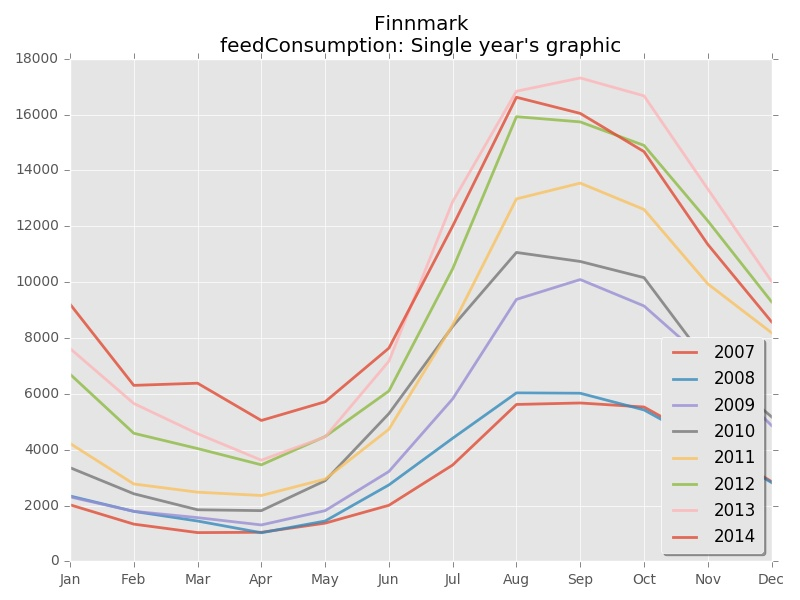
\includegraphics[trim={0 0 0 0},clip,width=1\textwidth]{Files/Finnmark_feedConsumption_years.jpg}
    \caption{Annual consumption of feed trend in Finnmark. }
    \label{fig: Finnmark_feed}
\end{figure}
\end{minipage} \hfill
\begin{minipage}[t]{0.60\textwidth}
\begin{figure}[H]
    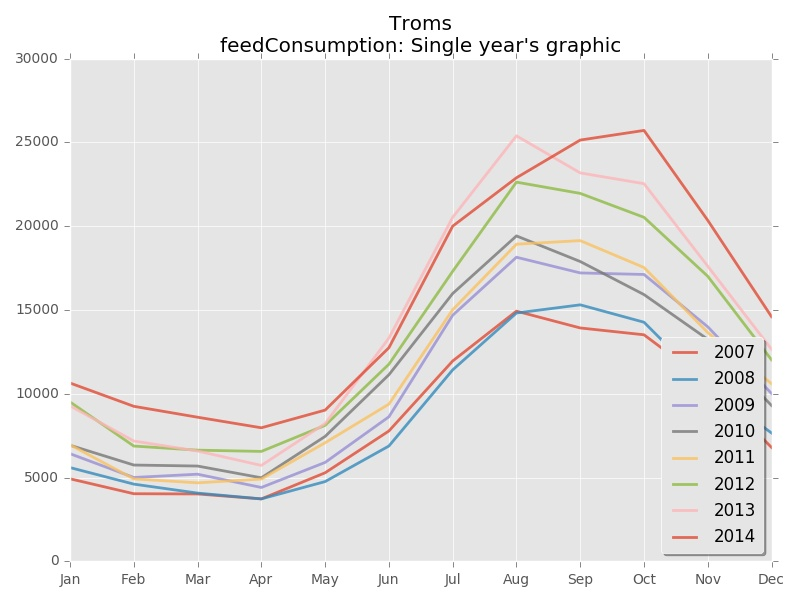
\includegraphics[trim={0 0 0 0},clip,width=1\textwidth]{Files/Troms_feedConsumption_years.jpg}
    \caption{Annual consumption of feed trend in Troms. }
    \label{fig: Troms_feed}
\end{figure}
\end{minipage}}
\makebox[1\textwidth][c]{
\begin{minipage}[t]{0.6\textwidth}
\begin{figure}[H]
    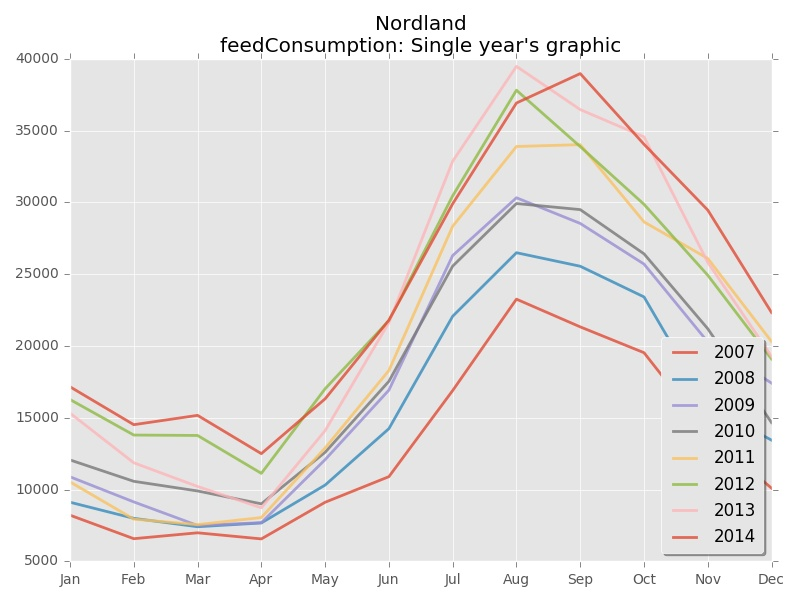
\includegraphics[trim={0 0 0 0},clip,width=1\textwidth]{Files/Nordland_feedConsumption_years.jpg}
    \caption{Annual consumption of feed trend in Nordland. }
    \label{fig: Nordland_feed}
\end{figure}
\end{minipage} \hfill
\begin{minipage}[t]{0.60\textwidth}
\begin{figure}[H]
    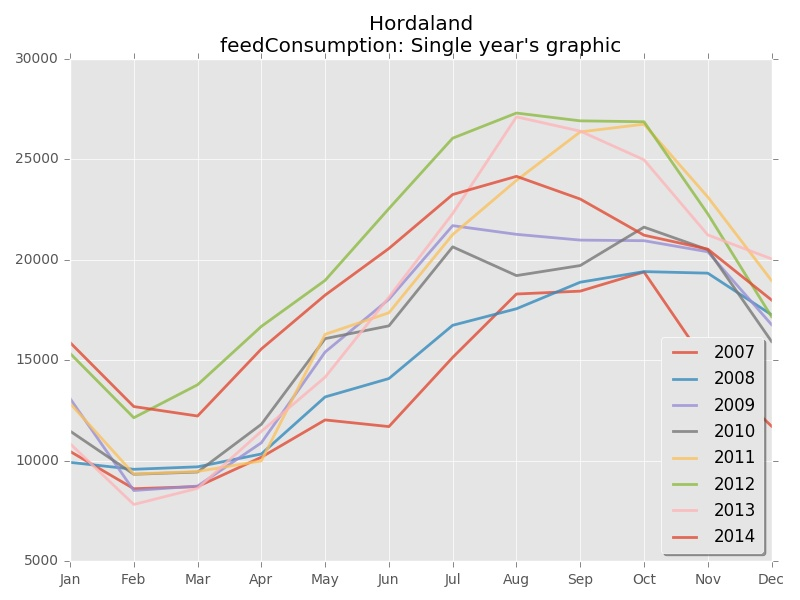
\includegraphics[trim={0 0 0 0},clip,width=1\textwidth]{Files/Hordaland_feedConsumption_years.jpg}
    \caption{Annual consumption of feed trend in Hordaland. }
    \label{fig: Hordaland_feed}
\end{figure}
\end{minipage}}


\makebox[1\textwidth][c]{
\begin{minipage}[t]{0.6\textwidth}
\begin{figure}[H]
    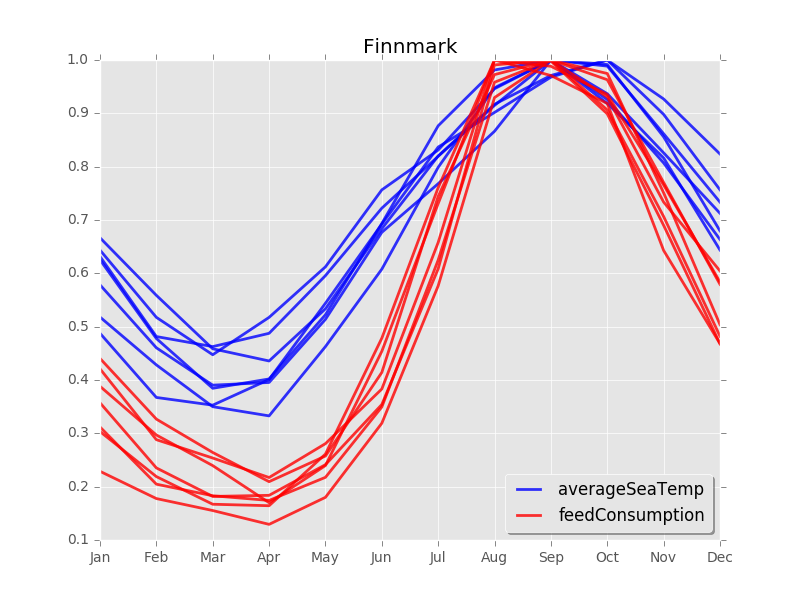
\includegraphics[trim={0 0 0 0},clip,width=1\textwidth]{Files/Finnmark-Temp&Feed.png}
    \caption{Comparison between average sea temperature and feed consumption in Finnmark}
    \label{fig: Finnmark_seaTemp&feed}
\end{figure}
\end{minipage} \hfill
\begin{minipage}[t]{0.6\textwidth}
\begin{figure}[H]
	\centering
    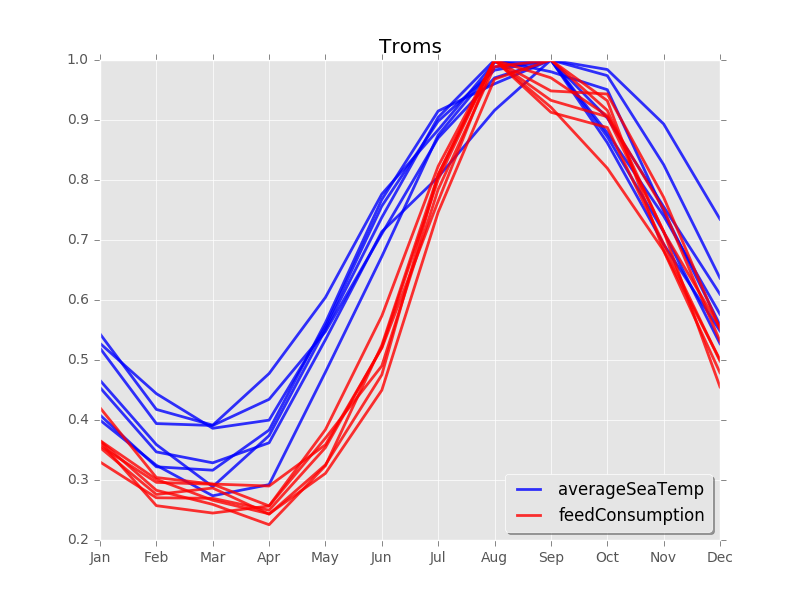
\includegraphics[trim={0 0 0 0},clip,width=1\textwidth]{Files/Troms-Temp&Feed.png}
    \caption{Comparison between average sea temperature and feed consumption in Troms}
    \label{fig: Troms_seaTemp&feed}
\end{figure}
\end{minipage}}
\makebox[1\textwidth][c]{
\begin{minipage}[t]{0.6\textwidth}
\begin{figure}[H]
    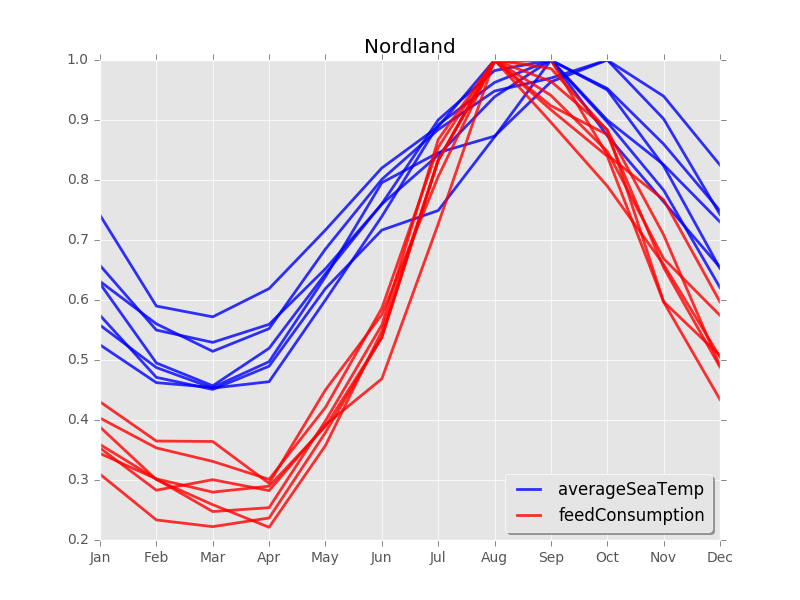
\includegraphics[trim={0 0 0 0},clip,width=1\textwidth]{Files/Nordland-Temp&Feed.png}
    \caption{Comparison between average sea temperature and feed consumption in Nordland}
    \label{fig: Nordland_seaTemp&feed}
\end{figure}
\end{minipage} \hfill
\begin{minipage}[t]{0.6\textwidth}
\begin{figure}[H]
	\centering
    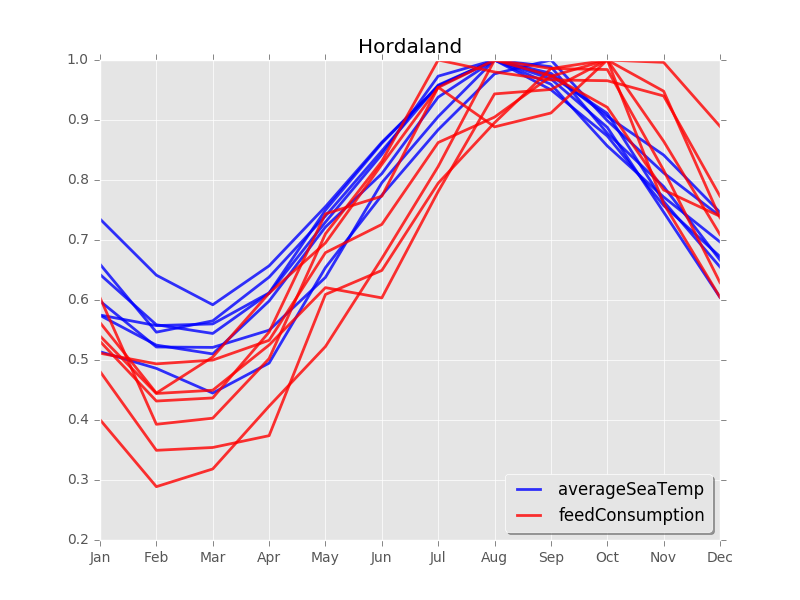
\includegraphics[trim={0 0 0 0},clip,width=1\textwidth]{Files/Hordaland-Temp&Feed.png}
    \caption{Comparison between average sea temperature and feed consumption in Hordaland}
    \label{fig: Hordaland_seaTemp&feed}
\end{figure}
\end{minipage}}



\begin{figure}[H]
	\makebox[\textwidth][c]{
    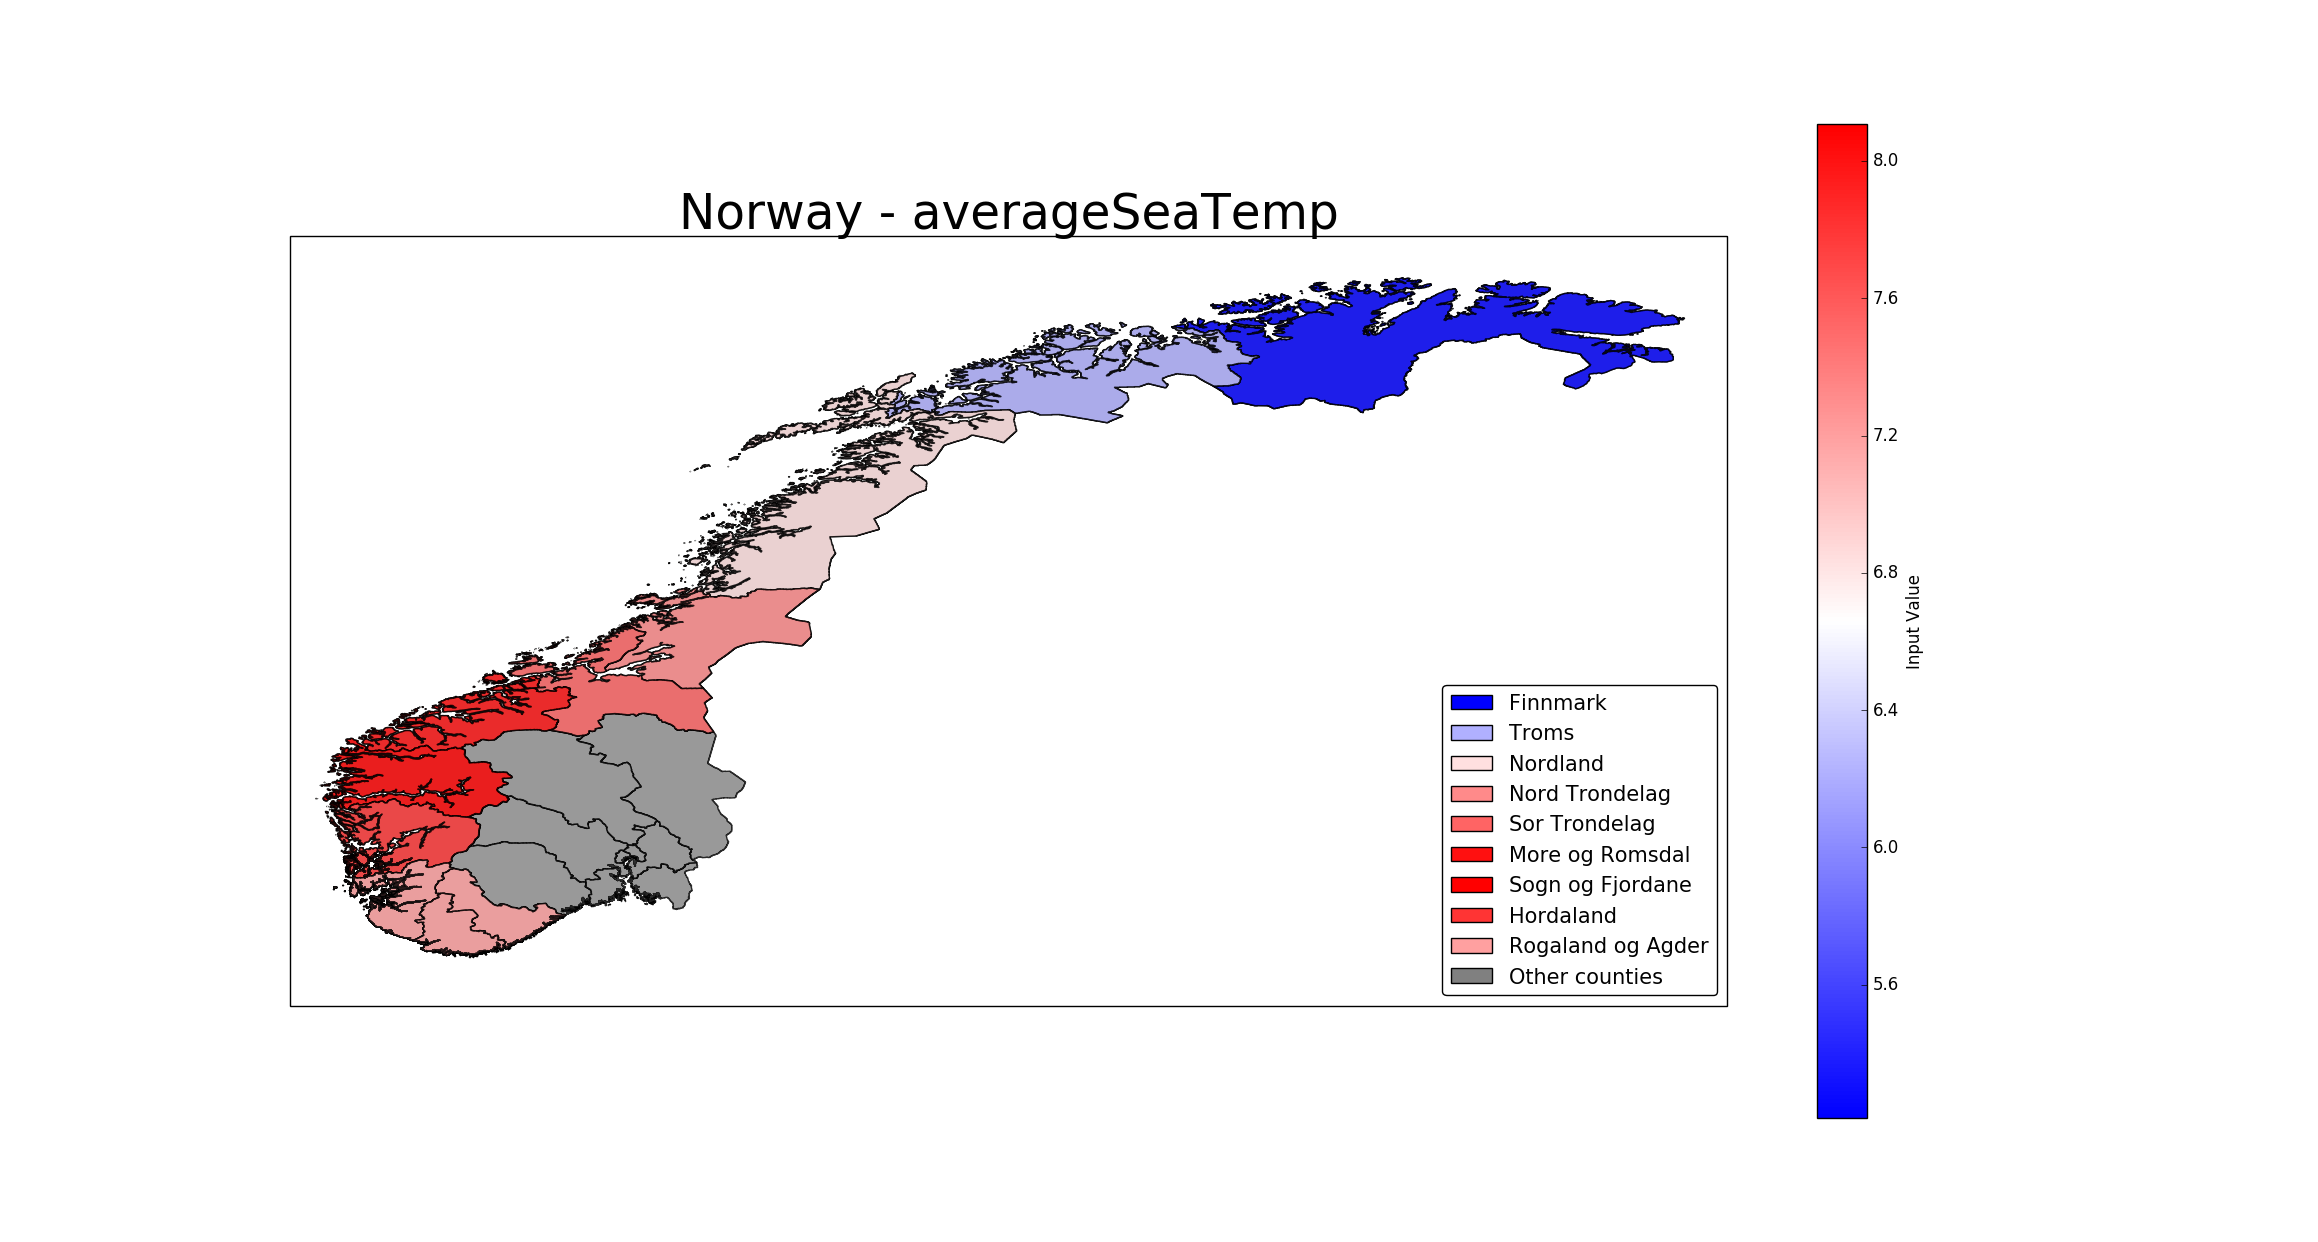
\includegraphics[trim={0 3cm 0 0},clip,width=1.3\textwidth]{Files/norway_averageSeaTemp.png}}
    \caption{Monthly average sea temperature from 200}
    \label{fig: Norway_averageSeaTemp}
\end{figure}

\begin{figure}[H]
	\makebox[\textwidth][c]{
    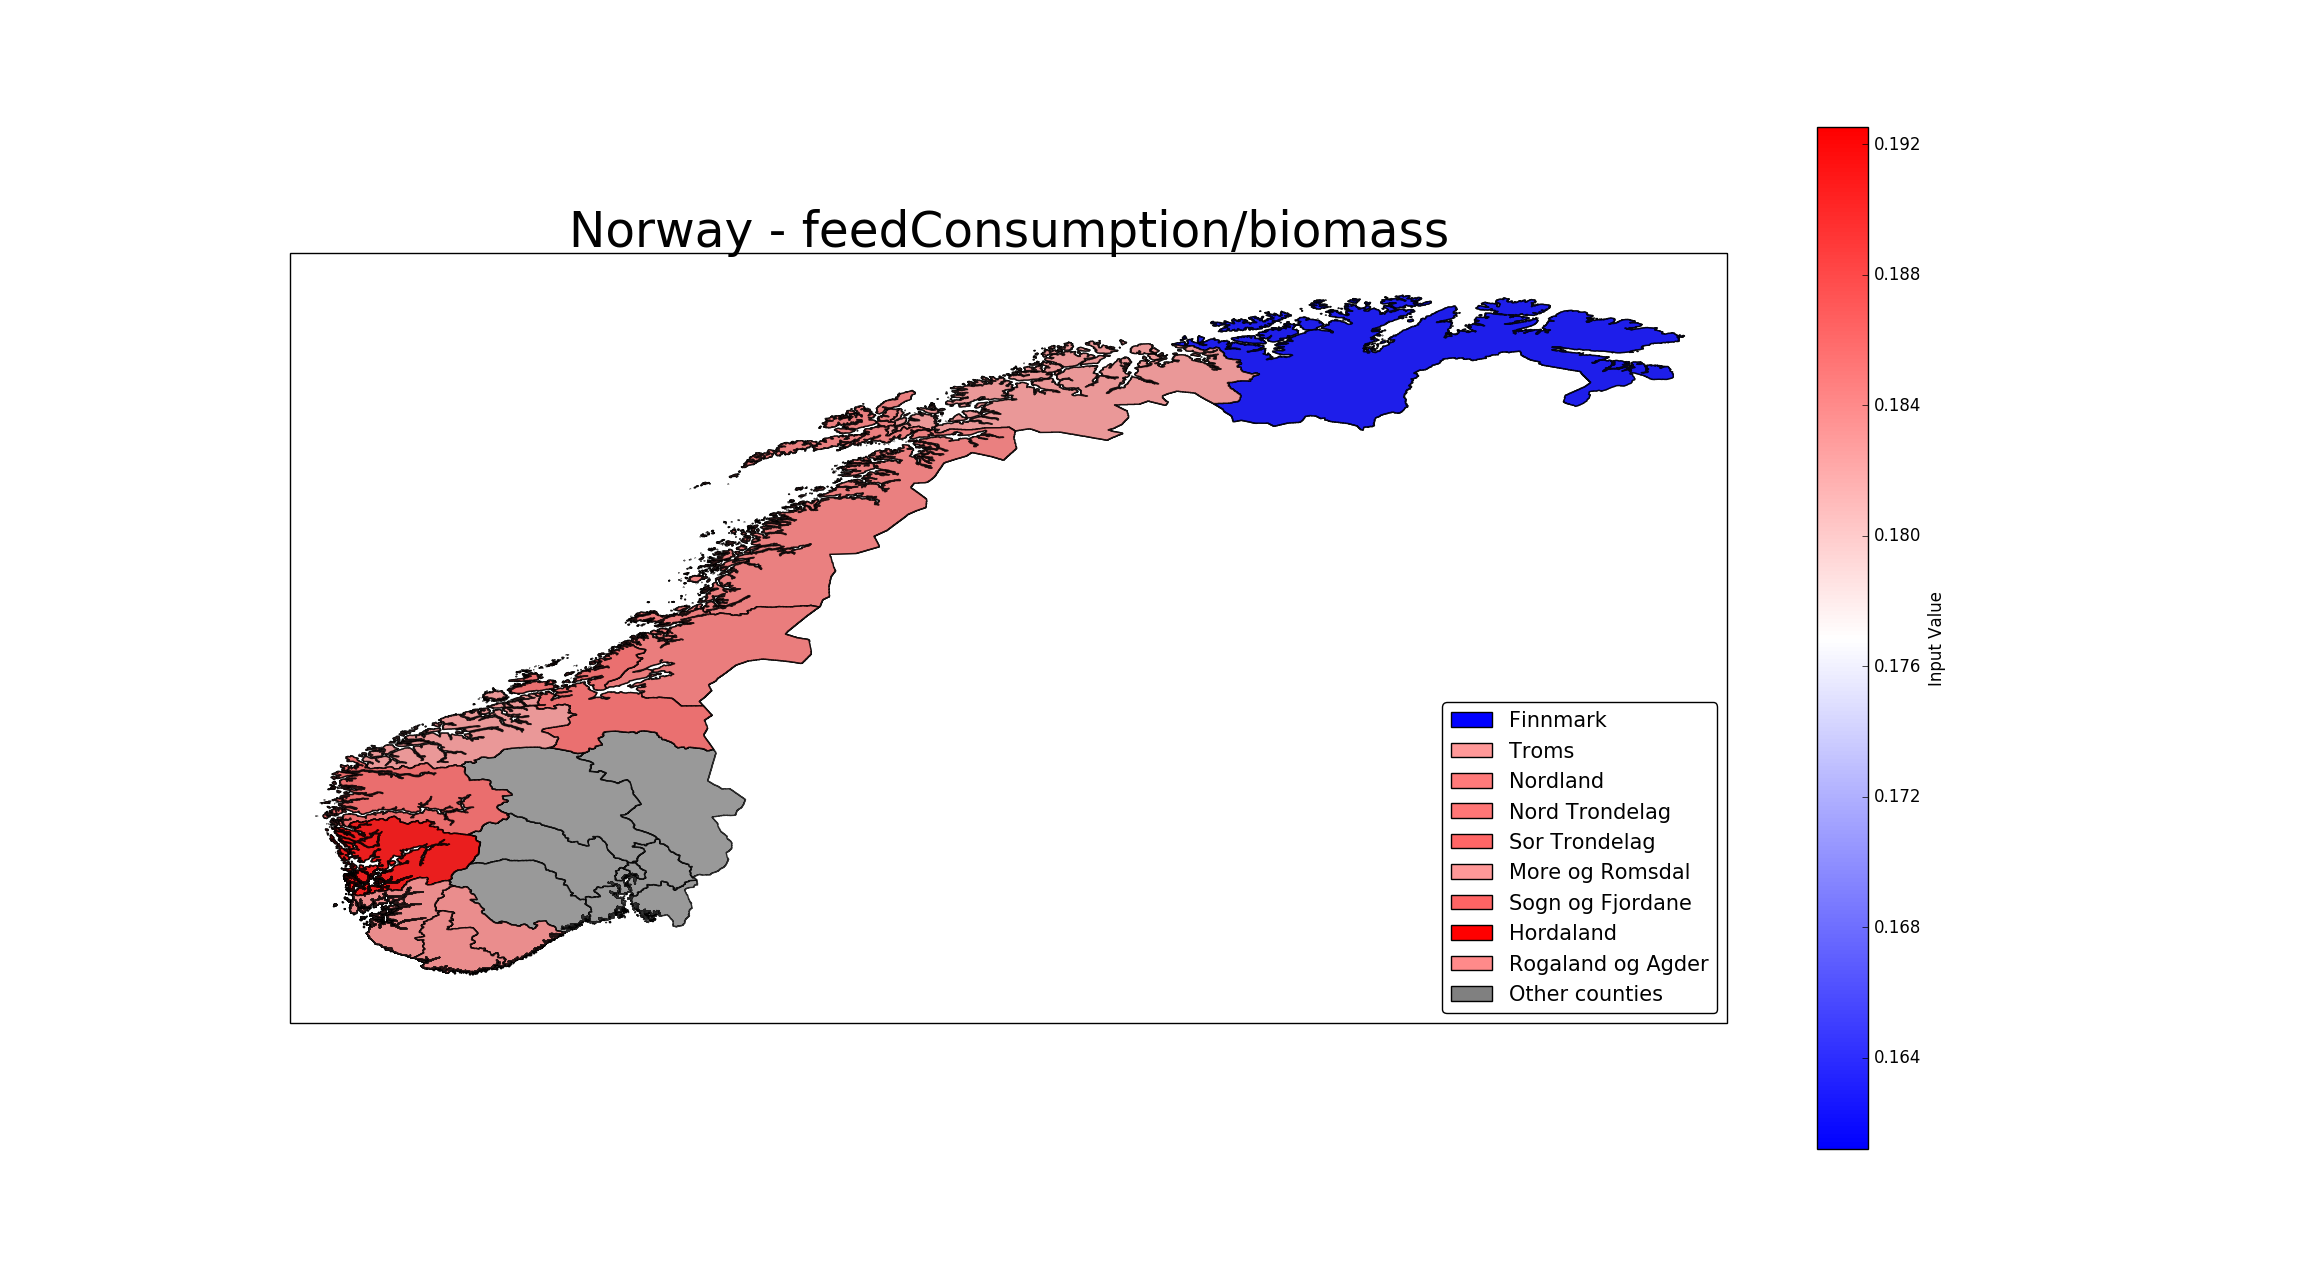
\includegraphics[trim={0 0 0 0},clip,width=1.3\textwidth]{Files/norway_feed-biomass.png}}
    \caption{Data science concept}
    \label{fig: Data_science}
\end{figure}



\section{Evaluation and limitations of the study}
\vspace{-5mm}
This study has a number of possible limitations, mainly due to a lack of background knowledge and experience about the current area, and also because of the relatively short time available.

ABOUT PYTHON RESULTS:
\vspace{-5mm}
\begin{itemize}
 \setlength{\itemsep}{-5pt}
\item PRO: The implemented Python system has a quite high reusability. It means that is possible to use it also with dataset filled with data parameter coming from other area of interest.
\item CONS: The implemented system in this thesis is probably efficient and productive for a personal use. That's because there is no GUI implemented and to change the customization of the output graphics you have to know Python language.
\item CONS: Not enough informations about machine learning field, so during this thesis was implemented just a basic implementation of the forecasting system, just to give an idea about how it works and give the possibility to improve it in future works.
\end{itemize}


ABOUT DATA ANALYSIS RESULTS:
\vspace{-5mm}
\begin{itemize}
 \setlength{\itemsep}{-5pt}
 \item PRO: Well structured datasets provided
 \item PRO: Usability of the results 
 \item CONS: Since the data sources are public, it's not possible to know the real reliability of it.
 \item CONS: The data collected are allowing just limitated analysis.
 \item CONS: Not enough informations have been extracted from the data cause of a lack in the background theory about Norwegian salmon farming, and not enough time to document myself in a proper way.
\end{itemize}


